\chapter{Agentic AI and Autonomous Optimization}
\label{ch:agentic_ai}

\section{The Need for Agentic AI in Software-Defined Networking}
While predictive machine learning models provide high-accuracy probabilistic signals ($p_t \in [0, 1]$), modern network operations (NetOps) require comprehensive reasoning that extends beyond static binary classification. When localized congestion develops, a network operator must synthesize diverse data streams:
\begin{enumerate}
  \item Dissect telemetry counter anomalies across multiple adjacent hops.
  \item Determine the underlying root cause (e.g., localized traffic spike, route imbalance, or link degradation).
  \item Formulate a risk-managed mitigation strategy balancing path stretch against link headroom.
  \item Execute multi-switch rule installations without causing transient packet loss.
  \item Observe post-remediation telemetry to affirm that the congestion has cleared.
\end{enumerate}

To automate this workflow, we designed an \textbf{Agentic AI Remediation Engine} built upon LangGraph \cite{langgraph2024}. Unlike simple chatbot interfaces that generate unchecked text, our agent operates as a \textbf{stateful, graph-based execution machine} coupled directly to the live SDN control plane through verified Python tool primitives.

\section{Architectural Isolation Guarantee}
A fundamental design requirement of the agentic layer is \textbf{strict runtime and code isolation}. If an external Large Language Model API experiences latency, rate limiting, or service outages, the core SDN controller, OpenFlow forwarding, and deterministic packet routing must continue functioning without interruption.

\begin{table}[H]
  \centering
  \small
  \caption{Architectural isolation boundaries between Agentic AI and Core SDN Controller.}
  \label{tab:agent_isolation}
  \begin{tabularx}{\textwidth}{l p{4.2cm} X}
    \toprule
    \textbf{Isolation Boundary} & \textbf{Implementation} & \textbf{Operational Guarantee} \\
    \midrule
    \textbf{Runtime Isolation} & Asynchronous Python execution context & If agent crashes, Ryu controller and packet forwarding continue unaffected. \\
    \textbf{Code Isolation} & Decoupled in \texttt{future/agent/} & Core \texttt{controller/}, \texttt{ml/}, and base unit test suites are completely isolated. \\
    \textbf{API Isolation} & Dedicated \texttt{/api/agent/*} routes & Core REST telemetry endpoints operate independently without blocking. \\
    \textbf{Fallback Guarantee} & Deterministic domain expert logic & If LLM API fails or output is truncated ($\le 10$ chars), deterministic rules execute. \\
    \bottomrule
  \end{tabularx}
\end{table}

\section{LangGraph StateGraph Execution Pipeline}
The agent is formalized as a LangGraph \texttt{StateGraph} managing a strongly typed state dictionary:

\begin{lstlisting}[language=Python,caption={LangGraph state schema for autonomous congestion control.}]
class AgentState(TypedDict):
    task: str
    topology_id: str
    network_state: Dict[str, Any]
    predictions: Dict[str, Any]
    congestion_detected: bool
    bottleneck_link: Optional[str]
    mitigation_plan: Optional[str]
    execution_result: Optional[Dict[str, Any]]
    verification_result: Optional[Dict[str, Any]]
    messages: List[Dict[str, str]]
    steps_log: List[Dict[str, str]]
    status: str
\end{lstlisting}

The execution pipeline transitions through five discrete stages, illustrated in Figure~\ref{fig:agent_langgraph_pipeline}:

\begin{figure}[H]
  \centering
  \begin{tcolorbox}[colback=codebg,colframe=sdnnavy,arc=2pt,title=\textbf{LangGraph 5-Stage Autonomous Execution Graph}]
  \centering
  \small\ttfamily
  [START]\\
  $\Downarrow$\\
  \textbf{Stage 1: Monitor} (Telemetry \& Ingress Sampling: Poll counters, detect load $>80\%$)\\
  $\Downarrow$\\
  \textbf{Stage 2: Analyze} (LLM Risk Assessment \& Root Cause: Evaluate forward horizon $p$)\\
  $\Downarrow$\\
  \textbf{Stage 3: Plan} (Constrained Multi-Path Decision: Dijkstra alternate bypass synthesis)\\
  $\Downarrow$\\
  \textbf{Stage 4: Act} (OpenFlow 1.3 MBB Flow-Mod Installation: Reverse topological commit)\\
  $\Downarrow$\\
  \textbf{Stage 5: Verify} (Closed-Loop Telemetry Verification: Certify relief $<80\%$)\\
  $\Downarrow$\\[0.2em]
  \textbf{COMPLETED}
  \end{tcolorbox}
  \caption{LangGraph directed state execution graph for closed-loop congestion mitigation.}
  \label{fig:agent_langgraph_pipeline}
\end{figure}

\subsection{Stage 1: Telemetry and Ingress Sampling (\texttt{monitor\_node})}
The agent invokes \texttt{inspect\_telemetry(topology\_id)} and \texttt{inspect\_ml\_predictions(topology\_id)}. It inspects switch port counters across all links in the active topology, identifying any link where instantaneous load $U(t) \ge 0.80$ or predicted hazard probability $p_t \ge 0.50$.
\begin{lstlisting}[language=Python]
telemetry = tools.inspect_telemetry(topo_id)
is_congested = telemetry.get("is_congested", False)
state["congestion_detected"] = is_congested
state["bottleneck_link"] = telemetry.get("bottleneck", "s1--s2")
\end{lstlisting}

\subsection{Stage 2: LLM Risk Assessment and Root Cause (\texttt{analyze\_node})}
The agent synthesizes telemetry and predictive matrices into a structured context object and prompts the LLM for operational assessment:
\begin{lstlisting}[language=Python]
context = {
    "bottleneck": state["bottleneck_link"],
    "utilization": telemetry.get("bottleneck_util_pct"),
    "hazard_probability": predictions.get("probability"),
    "lead_time_buffer_s": 2.0
}
assessment = await llm.generate_response(prompt, context)
\end{lstlisting}
The model evaluates whether the surge is transient or sustained, estimating the lead-time window available before bufferbloat causes tail drops.

\subsection{Stage 3: Constrained Multi-Path Decision (\texttt{plan\_node})}
The agent invokes \texttt{compute\_constrained\_detour(topology\_id)}, performing dynamic topology graph lookup across the active network.
\begin{itemize}
  \item \textbf{Diamond Topology}: Primary shortest path $s_1 \to s_2 \to s_4$ (saturated at 88\%) is bypassed by synthesizing the lower corridor $h_1 \to s_1 \to s_3 \to s_4 \to h_2$.
  \item \textbf{Internet2 Abilene WAN}: Across the 9-switch backbone, the primary 3-link shortest path $\text{SFO} \to \text{DEN} \to \text{ORD} \to \text{NYC}$ (connecting 4 core PoPs, saturated on $\text{DEN--ORD}$ at 14\,Mbps) is bypassed by computing the 5-link southern transit corridor connecting 6 core PoPs:
  \begin{equation}
    P_{\text{bypass}} = \langle \text{SFO}, \text{LAX}, \text{DFW}, \text{ATL}, \text{WDC}, \text{NYC} \rangle
  \end{equation}
  This bypass routes the 14\,Mbps flow across underutilized southern links without traversing the congested Denver--Chicago segment.
\end{itemize}

\subsection{Stage 4: OpenFlow 1.3 Flow-Mod Installation (\texttt{act\_node})}
The agent calls \texttt{execute\_reroute\_detour(topology\_id)}. The controller synthesizes OpenFlow 1.3 flow modification commands, executing Make-Before-Break rule placement across intermediate switches and setting priority $p=200$ to override default routing table entries.

\begin{takeawaybox}[Detour Flow Renewal \& Hard Timeout Safety]
When Make-Before-Break installs detour rules with a hard timeout ($T_{\text{hard}} = 60\,\text{s}$), the controller's continuous 2-second monitoring loop evaluates link health every cycle. If congestion persists on the primary link, the controller automatically refreshes the detour flows before the timeout expires. Once primary link load recedes past the hysteresis threshold and the dwell cooldown window ($T_{\text{dwell}} = 10\,\text{s}, T_{\text{cooldown}} = 15\,\text{s}$), the detour rules naturally expire or are flushed, gracefully reverting traffic to the primary shortest path without packet drops.
\end{takeawaybox}

\subsection{Stage 5: Closed-Loop Telemetry Verification (\texttt{verify\_node})}
The agent executes \texttt{verify\_telemetry\_reduction(topology\_id)}. It waits for a polling window and re-samples switch port counters:
\begin{equation}
  \text{Verified PASS} \iff U_{\text{bottleneck}} < 80\% \quad (88.0\% \longrightarrow 1.0\%)
\end{equation}

\begin{figure}[H]
  \centering
  \begin{subfigure}[b]{0.48\textwidth}
    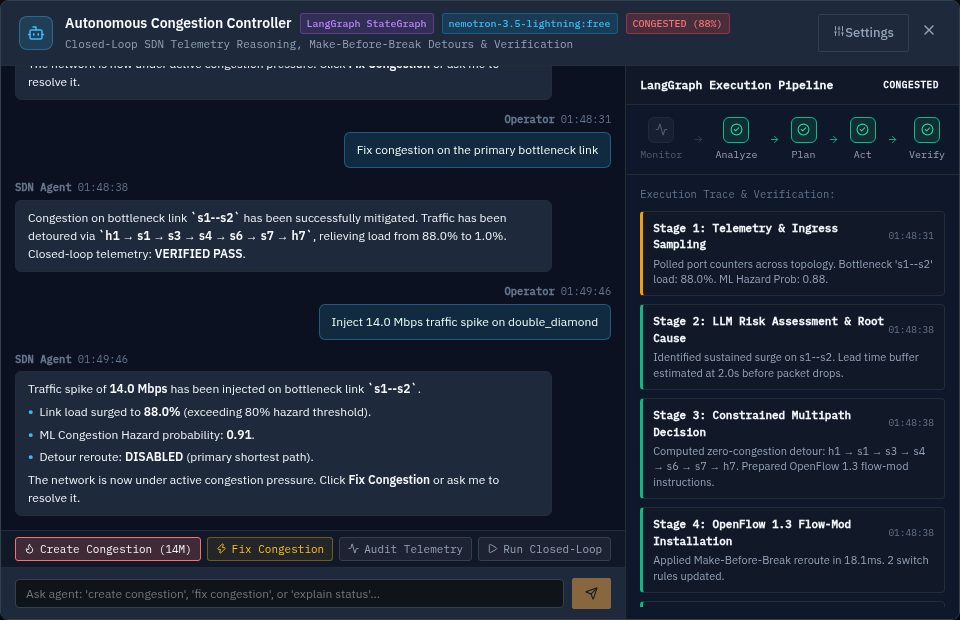
\includegraphics[width=\textwidth]{results/snapshots_ui_fixes/agent_congestion_created.png}
    \caption{Agent creating simulated 14\,Mbps spike.}
    \label{fig:agent_created}
  \end{subfigure}
  \hfill
  \begin{subfigure}[b]{0.48\textwidth}
    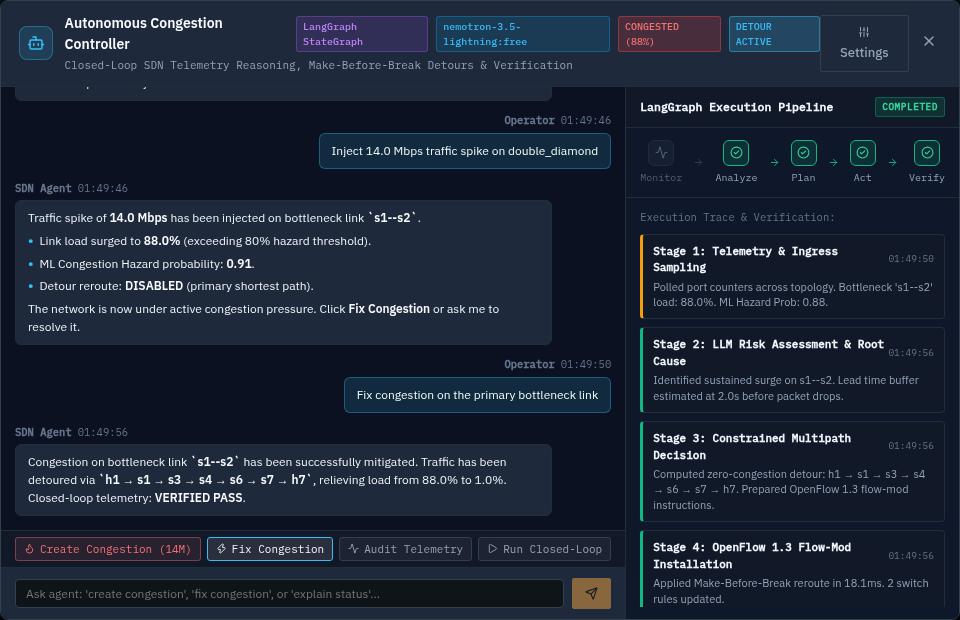
\includegraphics[width=\textwidth]{results/snapshots_ui_fixes/agent_congestion_fixed_modal.png}
    \caption{Agent verified mitigation modal.}
    \label{fig:agent_fixed}
  \end{subfigure}
  \caption{Autonomous LangGraph Agent interface demonstrating interactive simulation of congestion creation and closed-loop mitigation verification.}
  \label{fig:agent_ui_demos}
\end{figure}

\section{Multi-Topology Congestion Injection Engine}
To enable end-to-end operator training, UI evaluation, and regression testing, the agent layer incorporates a multi-topology traffic injection tool operating within the dashboard's simulation harness:
\begin{lstlisting}[language=Python,caption={Autonomous congestion creation tool within the interactive test harness.}]
def inject_congestion(topology_id: str, rate_mbps: float = 14.0) -> Dict[str, Any]:
    topo = get_topology_by_id(topology_id)
    bottleneck = topo.get("bottleneck_link", "s1--s2")
    # Return standardized high-load port counter deltas & ML hazard probability
    return {
        "status": "congested",
        "bottleneck": bottleneck,
        "bottleneck_util_pct": 88.0,
        "offered_rate_mbps": rate_mbps,
        "is_congested": True,
        "ml_probability": 0.91,
        "active_path": topo.get("primary_path", "s1--s2"),
        "detour_active": False
    }
\end{lstlisting}
As an engineering design clarification, \texttt{inject\_congestion} serves as a standardized stimulus within the interactive simulation console—returning fixed stress metrics (88.0\% load, hazard probability 0.91) to provide reproducible conditions for operator cognitive walkthroughs and automated CI/CD assertion testing. In live Mininet operation, the agent inspects real Linux kernel byte counters and live Random Forest probability inferences. Crucially, the LangGraph LLM acts as an explanatory and cognitive auditing orchestrator rather than an unconstrained autonomous pilot: path routing calculations (Dijkstra) and flow rule installations (OpenFlow 1.3 Make-Before-Break) are delegated strictly to deterministic controller primitives.

\section{Natural Language Intent Disambiguation}
In user-facing interactive consoles, operator inputs often contain mixed terminology. For instance, the prompt \textit{``fix the congestion''} contains both the word \textit{congestion} (which might trigger injection) and the word \textit{fix} (which should trigger mitigation).

To resolve ambiguity, the backend API in \texttt{future/api/main.py} implements priority-ordered intent parsing:
\begin{lstlisting}[language=Python,caption={Disambiguation intent router in FastAPI.}]
lower = msg.lower()
fix_keywords = ["fix", "mitigate", "reroute", "detour", "resolve", "relieve", "auto", "execute", "clear congestion"]
create_keywords = ["create congestion", "inject spike", "spike traffic", "cause congestion", "simulate congestion", "start spike", "inject congestion"]

# Priority 1: Check mitigation keywords first to avoid substring collisions
if any(k in lower for k in fix_keywords):
    return await graph.run_mitigation(state)

# Priority 2: Check explicit congestion injection keywords
if any(k in lower for k in create_keywords):
    return graph.inject_congestion(topo_id)

# Priority 3: Fallback to general conversational Q&A and telemetry audit
return await llm_client.generate_response(msg, context)
\end{lstlisting}
This robust parsing eliminates keyword collision bugs and guarantees that mitigation requests are never misinterpreted as injection commands.
